\begin{frame}\frametitle{Theory. Atom Structure}
\begin{figure}[htb]
  \begin{center}
    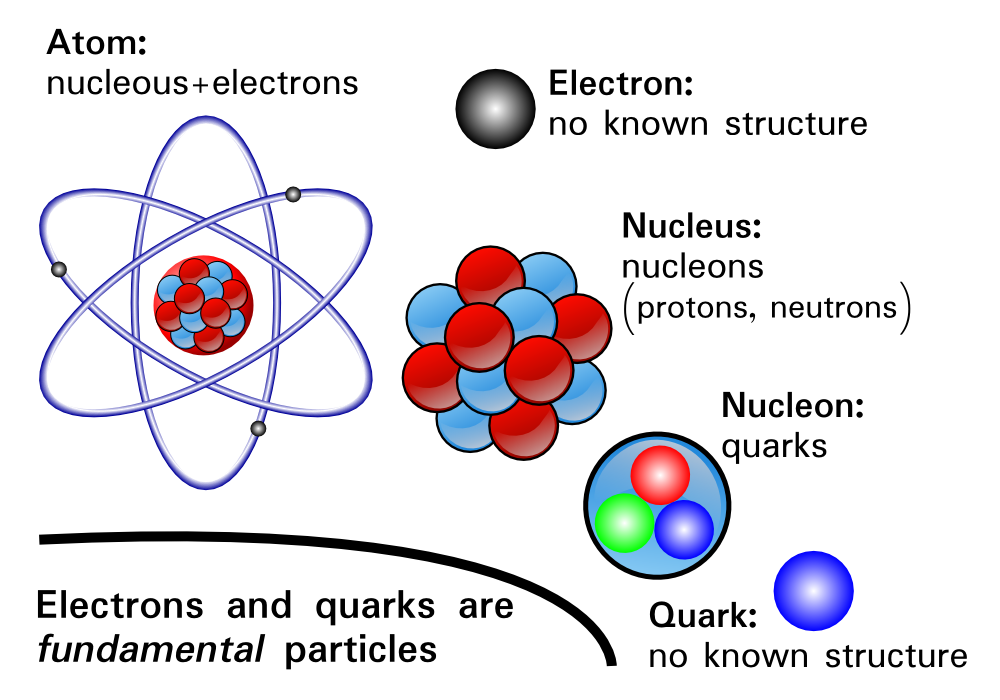
\includegraphics[width=0.98\textwidth]{../figs/ForPresentation/Theory_StandardModel01.png}
  \end{center}
\end{figure}
\end{frame}%{Atom Structure}

\begin{frame}\frametitle{Theory. The Standard Model}
\begin{figure}[htb]
  \begin{center}
    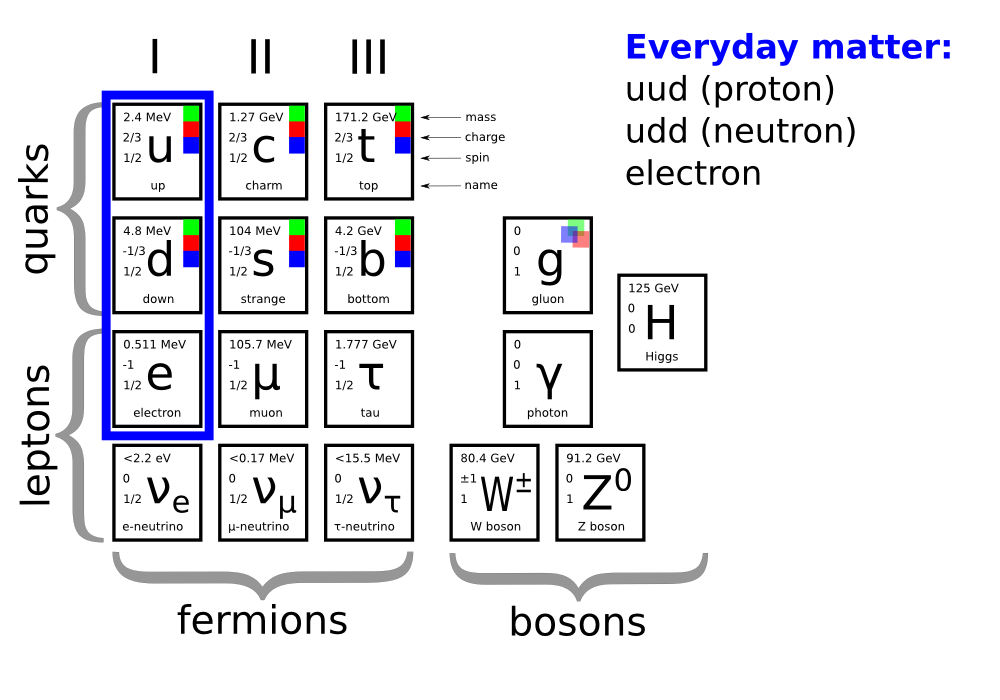
\includegraphics[width=0.98\textwidth]{../figs/ForPresentation/Theory_StandardModel02.png}
  \end{center}
\end{figure}
\end{frame}%{The Standard Model}

\begin{frame}\frametitle{Theory. Proton-Proton Collisions}
\begin{figure}[htb]
  \begin{center}
    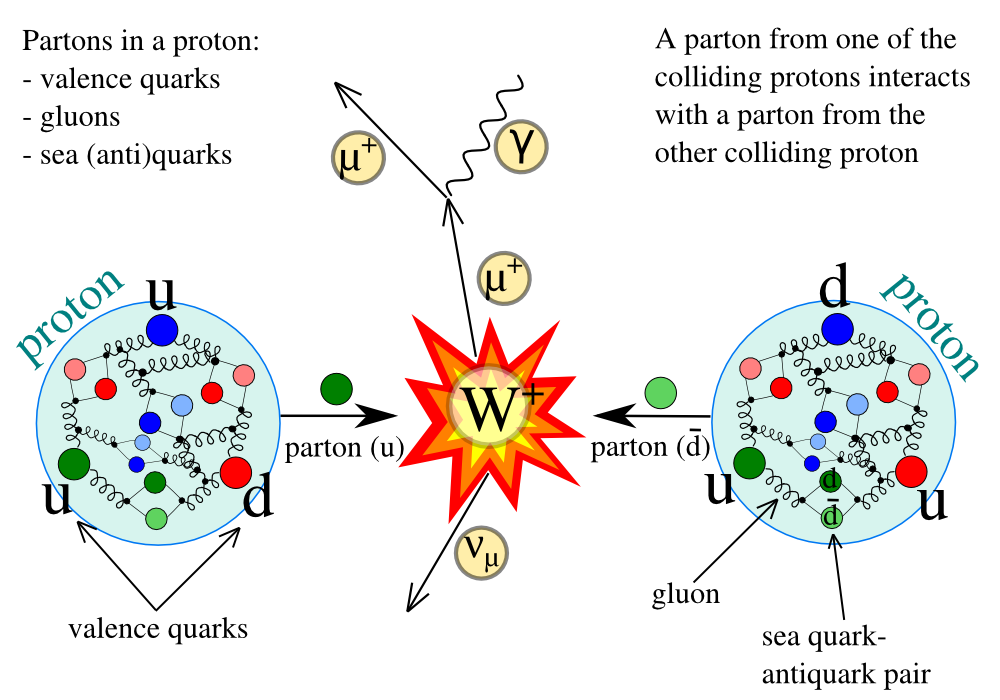
\includegraphics[width=0.95\textwidth]{../figs/ForPresentation/Theory_ppCollision.png}
  \end{center}
\end{figure}
\end{frame}%{Proton-Proton Collisions}

\begin{frame}\frametitle{Theory. $W\gamma\rightarrow l\nu\gamma$}
   \begin{figure}[htb]
      \begin{center}
        \scriptsize
          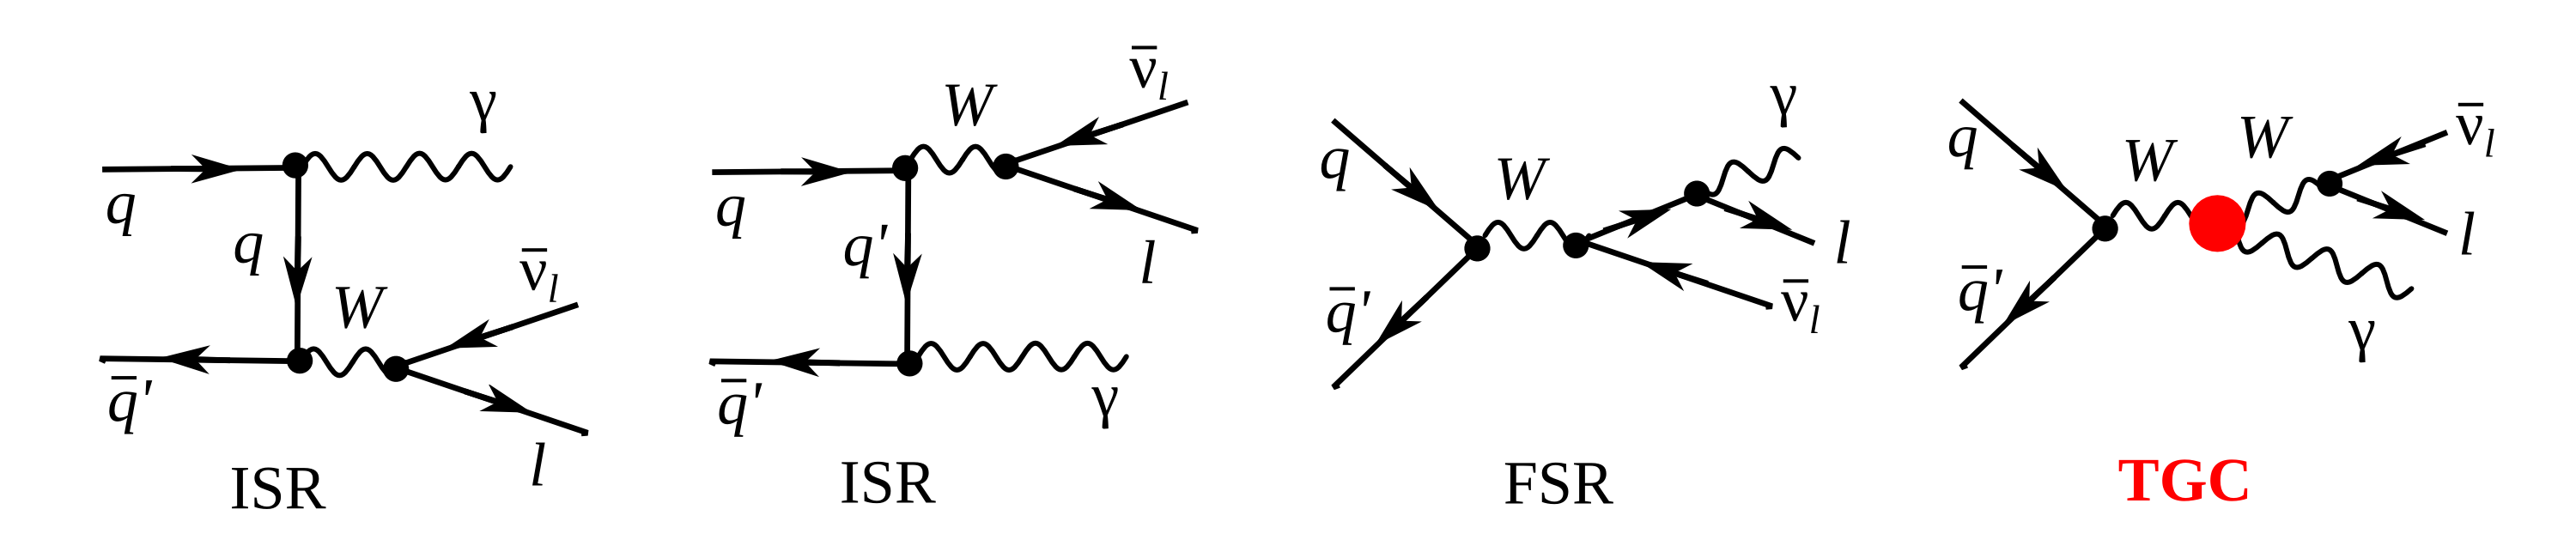
\includegraphics[width=0.95\textwidth]{../figs/ForPresentation/feynmWg_LO_02.png}
%          \caption{\scriptsize{The Feynman diagrams. ISR(x2), FSR, and TGC.}}
       \end{center}
    \end{figure}
\scriptsize
$q\bar{q'}\rightarrow W$ or $q\bar{q'}\rightarrow W\gamma$\\
-  \\
Usually $q\bar{q'}=u\bar{d}$ or  $q\bar{q'}=d\bar{u}$\\

\begin{table}[h]
  \scriptsize
  \begin{center}
   \begin{tabular}{|l|l|}
    \hline
         &  \\ 
     {\bfseries{Three mechanisms:}}  & {\bfseries{Measurement goals:}}  \\
         &  \\ 
     ISR: initial state radiation;   & Test the Standard Model;  \\ 
     FSR: final state radiation;    &  Provide a precise cross section measurement; \\ 
     {\color{red}{TGC: triple gauge coupling.}}    &  {\color{red}{Search for anomalous TGC (aTGC).}}\\ 
    &  \\  \hline
  \end{tabular}
  \end{center}
\end{table}

\end{frame}%{Theory. $W\gamma\rightarrow l\nu\gamma$}

